\documentclass[12pt]{article}
\usepackage{verbatim}
\usepackage[dvips]{epsfig}
\usepackage{color}
\usepackage{url}
\usepackage[colorlinks=true]{hyperref}

\begin{document}

\section*{GENESIS: Documentation}

{\bf Related Documentation:}
% start: userdocs-tag-replace-items related-do-nothing
% end: userdocs-tag-replace-items related-do-nothing

\section*{De Schutter: Purkinje Cell Model}

\begin{figure}[h]
\centering
   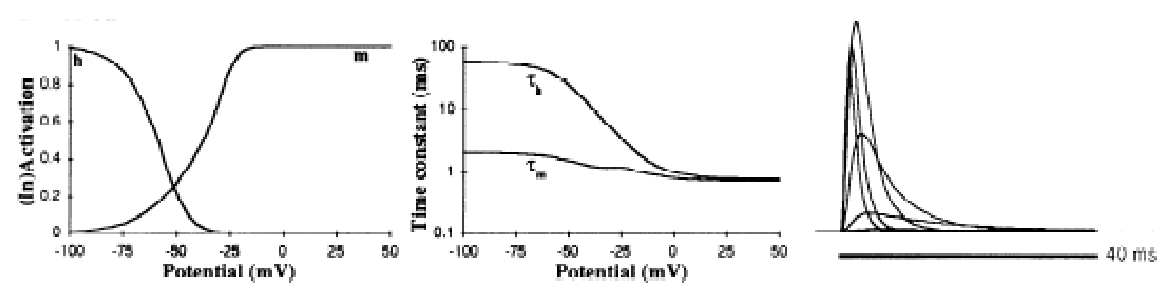
\includegraphics[scale=0.75]{figures/DS1.2F.eps}
   \caption{Activation and inactivation properties of the A current (KA, ---) in the model. Seady-state activation and inactivation vs. voltage are plotted at the {\em left}, the time constants of activation and inactivation($\tau_m$ and $\tau_h$) vs. voltage in the {\em middle} (Note: Semilogarithmic scale), and a simulation of representative voltage-clamp currents at the {\em right}, obtained from a spherical cell and assuming a complete block of all other channels. The voltage clamps simulate steps from a holding potential of -110 to -70\,mV up to 0\,mV in 10\,mV increments. The voltage-clamp current amplitude has been scaled arbitrarily because we mainly wanted to demonstrate the current kinetics.}
   \label{fig:DS1.2F}
\end{figure}

\subsection*{The A Current (KA)}

The presence of a conductance like an A current (KA) in the Purkinje cell was shown by\,\cite{Hounsgaard:1988nx}. We derived our equations for KA from the original reports on A currents\,\cite{Connor:1971tg, De-Schutter:1986hc} modified to fit the data in the two reports on Purkinje cell A currents that were available at that time. The whole cell voltage-clamp study of cultured Purkinje cells by\,\cite{Hirano:1989uq} (their Fig. 9) provided data about the activation and inactivation time constants and the steady-state inactivation, and a single-electrode voltage-clamp study in slice by\,\cite{Li:1990ij} supplied steady-state activation data.

Recently\,\cite{Wang:1991bs} published a more complete report on a single-electrode voltage-clamp study of the Purkinje cell. The average threshold for activation they report is lower than the value used in our model, but there seems to be a large natural variability in the activation curves (compare their Fig. 1 with their Table 1). The steady-state inactivation curve of\,\cite{Wang:1991bs} is similar to ours and to the kinetics of A currents in other systems\,\cite{Connor:1971tg, Rogawski:1985fv} but they report a much slower inactivation time constant than\,\cite{Hirano:1989uq}.

One point of contention in the literature about the 
distribution of ionic channels involves the presence
or absence of an A current in the distal dendrites\,\cite{Chan:1988fk, Hounsgaard:1988nx}.
One argument for a more extensive distribution is that a depolarizing
bias current, which would inactivate A currents,
also causes the dendrite to fire spikes more easily. However,
a similar result would be expected if the depolarization also
activated a plateau current, as shown in Fig. 11. Moreover,
in contrast to the expected 4-aminopyridine (4-AP) sensitivity
of A currents\,\cite{Rogawski:1985fv}, the outward current
described by\,\cite{Hounsgaard:1988nx} was not
blocked by 4-AP. In addition, voltage-clamp data\,\cite{Wang:1991bs} 
do not support a distal dendritic location of the A
current. Patch-clamp studies of cultured Purkinje cells\,\cite{Gruol:1991dz}
have shown the A current to be present
in both somatic and dendritic membrane, but it is likely
that patches were obtained from smooth dendrites only. In
the current model an A current was present in the soma and
main dendrite. However, dendritic spiking was more influenced
by the K2 Ca$^{2+}$ -activated K$^+$ current, which allowed
a finer control of dendritic excitability than the A
current, which inactivated quickly during long current injections.

\bibliographystyle{plain}
\bibliography{../tex/bib/g3-refs}

\end{document}
